\documentclass[11pt,compress,t,notes=noshow, xcolor=table]{beamer}
\usepackage[]{graphicx}\usepackage[]{color}
% maxwidth is the original width if it is less than linewidth
% otherwise use linewidth (to make sure the graphics do not exceed the margin)
\makeatletter
\def\maxwidth{ %
  \ifdim\Gin@nat@width>\linewidth
    \linewidth
  \else
    \Gin@nat@width
  \fi
}
\makeatother

\newcommand{\citebutton}[2]{%
\beamergotobutton{\href{#2}{#1}}%
}

\newcommand{\blu}[1]{\textcolor{blue}{#1}}
\newcommand{\org}[1]{\textcolor{orange}{#1}}
\newcommand{\ques}{\textbf{\textcolor{red}{Question:  }}}
\newcommand{\questionssofar}{\begin{frame}\frametitle{Any questions?}\end{frame}}

\newcommand\warning{%
 \makebox[1.4em][c]{%
 \makebox[0pt][c]{\raisebox{.1em}{\scriptsize!}}%
 \makebox[0pt][c]{\color{red}\normalsize$\bigtriangleup$}}}%

\definecolor{fgcolor}{rgb}{0.345, 0.345, 0.345}
\newcommand{\hlnum}[1]{\textcolor[rgb]{0.686,0.059,0.569}{#1}}%
\newcommand{\hlstr}[1]{\textcolor[rgb]{0.192,0.494,0.8}{#1}}%
\newcommand{\hlcom}[1]{\textcolor[rgb]{0.678,0.584,0.686}{\textit{#1}}}%
\newcommand{\hlopt}[1]{\textcolor[rgb]{0,0,0}{#1}}%
\newcommand{\hlstd}[1]{\textcolor[rgb]{0.345,0.345,0.345}{#1}}%
\newcommand{\hlkwa}[1]{\textcolor[rgb]{0.161,0.373,0.58}{\textbf{#1}}}%
\newcommand{\hlkwb}[1]{\textcolor[rgb]{0.69,0.353,0.396}{#1}}%
\newcommand{\hlkwc}[1]{\textcolor[rgb]{0.333,0.667,0.333}{#1}}%
\newcommand{\hlkwd}[1]{\textcolor[rgb]{0.737,0.353,0.396}{\textbf{#1}}}%
\let\hlipl\hlkwb

\usepackage{framed}
\makeatletter
\newenvironment{kframe}{%
 \def\at@end@of@kframe{}%
 \ifinner\ifhmode%
  \def\at@end@of@kframe{\end{minipage}}%
  \begin{minipage}{\columnwidth}%
 \fi\fi%
 \def\FrameCommand##1{\hskip\@totalleftmargin \hskip-\fboxsep
 \colorbox{shadecolor}{##1}\hskip-\fboxsep
     % There is no \\@totalrightmargin, so:
     \hskip-\linewidth \hskip-\@totalleftmargin \hskip\columnwidth}%
 \MakeFramed {\advance\hsize-\width
   \@totalleftmargin\z@ \linewidth\hsize
   \@setminipage}}%
 {\par\unskip\endMakeFramed%
 \at@end@of@kframe}
\makeatother

\definecolor{shadecolor}{rgb}{.97, .97, .97}
\definecolor{messagecolor}{rgb}{0, 0, 0}
\definecolor{warningcolor}{rgb}{1, 0, 1}
\definecolor{errorcolor}{rgb}{1, 0, 0}
\newenvironment{knitrout}{}{} % an empty environment to be redefined in TeX

\usepackage{alltt}
\newcommand{\SweaveOpts}[1]{}  % do not interfere with LaTeX
\newcommand{\SweaveInput}[1]{} % because they are not real TeX commands
\newcommand{\Sexpr}[1]{}       % will only be parsed by R
\newcommand{\xmark}{\ding{55}}%


\usepackage[english]{babel}
\usepackage[utf8]{inputenc}

\usepackage{dsfont}
\usepackage{verbatim}
\usepackage{amsmath}
\usepackage{amsfonts}
\usepackage{amssymb}
\usepackage{bm}
\usepackage{csquotes}
\usepackage{multirow}
\usepackage{longtable}
\usepackage{booktabs}
\usepackage{enumerate}
\usepackage[absolute,overlay]{textpos}
\usepackage{psfrag}
\usepackage{algorithm}
\usepackage{algpseudocode}
\usepackage{eqnarray}
\usepackage{arydshln}
\usepackage{tabularx}
\usepackage{placeins}
\usepackage{tikz}
\usepackage{setspace}
\usepackage{colortbl}
\usepackage{mathtools}
\usepackage{wrapfig}
\usepackage{bm}
\usepackage{amsmath}
\usepackage{pifont}

\usetikzlibrary{shapes.multipart,shapes,arrows,automata,positioning,calc,chains,trees, shadows}
\tikzset{
  %Define standard arrow tip
  >=stealth',
  %Define style for boxes
  punkt/.style={
    rectangle,
    rounded corners,
    draw=black, very thick,
    text width=6.5em,
    minimum height=2em,
    text centered},
  % Define arrow style
  pil/.style={
    ->,
    thick,
    shorten <=2pt,
    shorten >=2pt,}
}

\tikzstyle{vec}=[draw, rectangle, fill = white, minimum width=5mm, minimum height=1cm, inner sep = 2pt]

\usepackage{subfig}

% Defines macros and environments
\usepackage{../../style/lmu-lecture}


\let\code=\texttt
\let\proglang=\textsf

\setkeys{Gin}{width=0.9\textwidth}

\setbeamertemplate{frametitle}{\expandafter\uppercase\expandafter\insertframetitle}

\usepackage{bbm}
% basic latex stuff
\newcommand{\pkg}[1]{{\fontseries{b}\selectfont #1}} %fontstyle for R packages
\newcommand{\lz}{\vspace{0.5cm}} %vertical space
\newcommand{\dlz}{\vspace{1cm}} %double vertical space
\newcommand{\oneliner}[1] % Oneliner for important statements
{\begin{block}{}\begin{center}\begin{Large}#1\end{Large}\end{center}\end{block}}


%new environments
\newenvironment{vbframe}  %frame with breaks and verbatim
{
 \begin{frame}[containsverbatim,allowframebreaks]
}
{
\end{frame}
}

\newenvironment{vframe}  %frame with verbatim without breaks (to avoid numbering one slided frames)
{
 \begin{frame}[containsverbatim]
}
{
\end{frame}
}

\newenvironment{blocki}[1]   % itemize block
{
 \begin{block}{#1}\begin{itemize}
}
{
\end{itemize}\end{block}
}

\newenvironment{fragileframe}[2]{  %fragile frame with framebreaks
\begin{frame}[allowframebreaks, fragile, environment = fragileframe]
\frametitle{#1}
#2}
{\end{frame}}


\newcommand{\myframe}[2]{  %short for frame with framebreaks
\begin{frame}[allowframebreaks]
\frametitle{#1}
#2
\end{frame}}

\newcommand{\remark}[1]{
  \textbf{Remark:} #1
}


\newenvironment{deleteframe}
{
\begingroup
\usebackgroundtemplate{
\includegraphics[width=\paperwidth,height=\paperheight]{../style/color/red.png}}
 \begin{frame}
}
{
\end{frame}
\endgroup
}
\newenvironment{simplifyframe}
{
\begingroup
\usebackgroundtemplate{
\includegraphics[width=\paperwidth,height=\paperheight]{../style/color/yellow.png}}
 \begin{frame}
}
{
\end{frame}
\endgroup
}\newenvironment{draftframe}
{
\begingroup
\usebackgroundtemplate{
\includegraphics[width=\paperwidth,height=\paperheight]{../style/color/green.jpg}}
 \begin{frame}
}
{
\end{frame}
\endgroup
}
% https://tex.stackexchange.com/a/261480: textcolor that works in mathmode
\makeatletter
\renewcommand*{\@textcolor}[3]{%
  \protect\leavevmode
  \begingroup
    \color#1{#2}#3%
  \endgroup
}
\makeatother





\input{../../latex-math/basic-math.tex}
\input{../../latex-math/basic-ml.tex}

\newcommand{\titlefigure}{figure/bertology.png}
\newcommand{\learninggoals}{
\item Understand how impactful this architecture was
\item See how this changed research in the field
\item Glimpse into BERTology}

\title{Post-BERT Era}
% \author{}
\institute{\href{https://slds-lmu.github.io/lecture_dl4nlp/}{slds-lmu.github.io/lecture\_dl4nlp}}
\date{}

\begin{document}
\lecturechapter{Implications for future work \& BERTology}
\lecture{Deep Learning for NLP}

% ------------------------------------------------------------------------------

\begin{frame}{Implications / Limitations}

\vfill

	\begin{itemize}
		\item BERT changed the way NLP research was done over night\\
					(probably as impactful as ChatGPT in 2022, but not so incredibly hyped in the general public)
		\item This paradigm change had several \myblue{implications} on how research was done in the ``Post-BERT era``
		\item It also came with several \myblue{limitations} that are still to be solved or have been solved already
		\item Computational power also became an important issue, but this will not be stressed as much in this chapter
	\end{itemize}

\vfill

\end{frame}

% ------------------------------------------------------------------------------

\begin{frame}{(1) language diversity}

\vfill

	\begin{itemize}
		\item BERT trained on a corpus of English text
		\item More importantly: Also only evaluated on English benchmarks (obviously)
					\citebutton{GLUE}{https://gluebenchmark.com/}
					\citebutton{SQUAD}{https://rajpurkar.github.io/SQuAD-explorer/}
					\citebutton{RACE}{https://www.qizhexie.com/data/RACE_leaderboard.html}
		\item Devlin et al. (2019) published different (monolingual) models, but only varying in size, not in language
		\item Later: Multilingual BERT model \citebutton{mBERT}{https://github.com/google-research/bert/blob/master/multilingual.md} for 100+ languages
		\item This leads to a shared embedding space for all the languages included in the model
		\item Before this: Need for alignment of separately learned embedding spaces
	\end{itemize}

\vfill

\end{frame}

% ------------------------------------------------------------------------------

\begin{frame}{(1) language diversity}

\vfill

\begin{itemize}
	\item The breakthrough performance of BERT in the English language triggered a wave of new
				BERT models in different languages. Just to name a few:
			\begin{itemize}
				\item \citebutton{German BERT}{https://huggingface.co/bert-base-german-cased}
				\item \citebutton{FlauBERT (French)}{https://huggingface.co/flaubert/flaubert_base_cased}
				\item \citebutton{BETO (Spanish)}{https://huggingface.co/dccuchile/bert-base-spanish-wwm-cased}
				\item \citebutton{BERTje (Dutch)}{https://huggingface.co/GroNLP/bert-base-dutch-cased}
				\item \citebutton{Chinese BERT}{https://huggingface.co/bert-base-chinese}
				\item \citebutton{RuBERT (Russian)}{https://huggingface.co/DeepPavlov/rubert-base-cased}
				\item \citebutton{Italian BERT}{https://huggingface.co/dbmdz/bert-base-italian-cased}
				\item ...
			\end{itemize}
\end{itemize}
	
\vfill

\end{frame}

% ------------------------------------------------------------------------------

\begin{frame}{(2) pretrain-finetune + transformer}

\vfill

\textbf{Before BERT:} 
			\begin{itemize}
				\item ELMo (and other specialized architectures) very popular
				\item Examples (also CNNs): 
							\citebutton{Kim, 2014}{https://arxiv.org/abs/1408.5882}
							\citebutton{Zhang et al., 2016}{https://proceedings.neurips.cc/paper/2015/file/250cf8b51c773f3f8dc8b4be867a9a02-Paper.pdf}
			\end{itemize}
\textbf{After BERT:}
			\begin{itemize}
				\item Using a pre-trained model and fine-tuning it to one's own data is* the de-facto standard
				\item CNNs and RNNs rarely used, different variants of the transformer or other self-attention based mechanisms are the backbone of nearly every architecture
			\end{itemize}

\vfill

{\scriptsize *Or probably ``\textit{was}``. This standard is (rapidly) changing at the moment as Large Language Models (LLMs) and Prompting are becoming incredibly popular and effective.}
\end{frame}

% ------------------------------------------------------------------------------

\begin{frame}{(3) pretrain-finetune discrepancy}

\vfill

	\begin{itemize}
		\item BERT \textit{artificially} introduces \texttt{[MASK]} tokens during pre-training
		\item \texttt{[MASK]}-token does not occur during fine-tuning\\
					$\rightarrow$ Lacks the ability to model joint probabilities\\
					$\rightarrow$ Assumes independence of predicted tokens (given the context)
		\item Other pre-training objectives (e.g. language modeling) don't have this issue
		\item Further: BERT only learns from predicting the 15\% tokens which are \texttt{[MASK]}ed (or randomly replaced / kept as is)
	\end{itemize}

\vfill

\end{frame}

% ------------------------------------------------------------------------------

\begin{frame}{(4) independence assumption}

\vspace{1.5cm}

\textbf{\texttt{[MASK]-ing procedure}:}

\begin{itemize}
	\item "Given a sentence, predict \texttt{[MASK]}ed tokens"
	\item All \texttt{[MASK]}ed tokens are predicted based on the un-\texttt{[MASK]}ed tokens
	\item \textit{Implicit assumption:} Independence of \texttt{[MASK]}ed tokens
\end{itemize}

	\begin{figure}
		\centering
		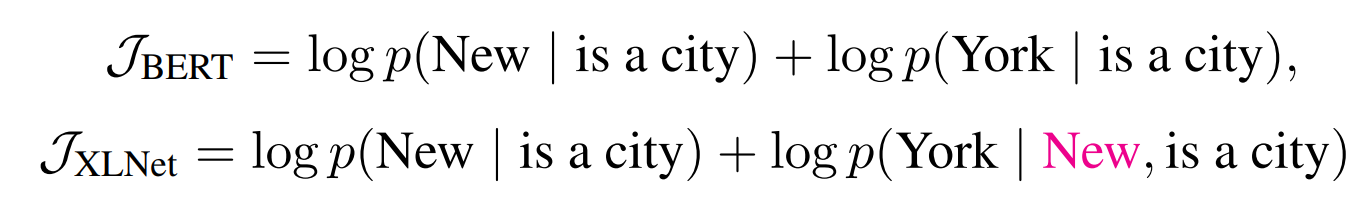
\includegraphics[width = 9cm]{figure/xlnet-objective}\\ 
		{\tiny Prediction of [New, York] given the factorization order [is, a, city, New, York]}\\
		\citebutton{Source: Yang et al., 2019}{https://papers.nips.cc/paper_files/paper/2019/hash/dc6a7e655d7e5840e66733e9ee67cc69-Abstract.html}
	\end{figure}
	
\end{frame}

% ------------------------------------------------------------------------------

\begin{frame}{(5) maximum sequence length}

\begin{figure}
\centering
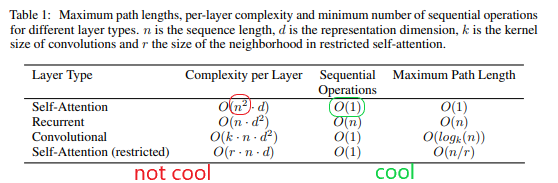
\includegraphics[width = 8.5cm]{figure/bert-problem.png}\\ 
	\beamergotobutton{\href{https://arxiv.org/abs/1706.03762}{Source: Vaswani et al., 2017}}
\end{figure}

\textbf{Limitation:}

\begin{itemize}
	\item BERT can only consume sequences of up to 512 tokens
	\item Two sentences for NSP are sampled such that $$length_{sentence A} + length_{sentence B} \leq 512$$
	\item Reason: Computational complexity of Transformer scales quadratically with the sequence length\\
				$\rightarrow$ Longer sequences are disproportionally expensive
\end{itemize}

\end{frame}

% ------------------------------------------------------------------------------

\begin{frame}{(6) bias}

\vfill

\begin{itemize}
	\item Already known to exist in static pre-trained embeddings:
	\item[] \textit{Man is to Computer Programmer as Woman is to Homemaker? Debiasing Word Embeddings} \citebutton{Bolukbasi et al., 2016}{https://arxiv.org/abs/1607.06520}
	\item BERT also learns the patterns from the data it is trained on
	\item Research on Detecting/Mitigating Bias receives a lot of attention
\end{itemize}


\vfill

\end{frame}

% ------------------------------------------------------------------------------

\begin{frame}{(6) bias -- example}

\vfill

\begin{itemize}
	\item \citebutton{Nadeem et al., 2021}{https://aclanthology.org/2021.acl-long.416.pdf} create a data set for measuring bias in LMs
	\item Four categories: Gender, Profession, Race, Religion
	\item Two types of probes: Intra- and Inter-sentence test sets
\end{itemize}

\begin{figure}%
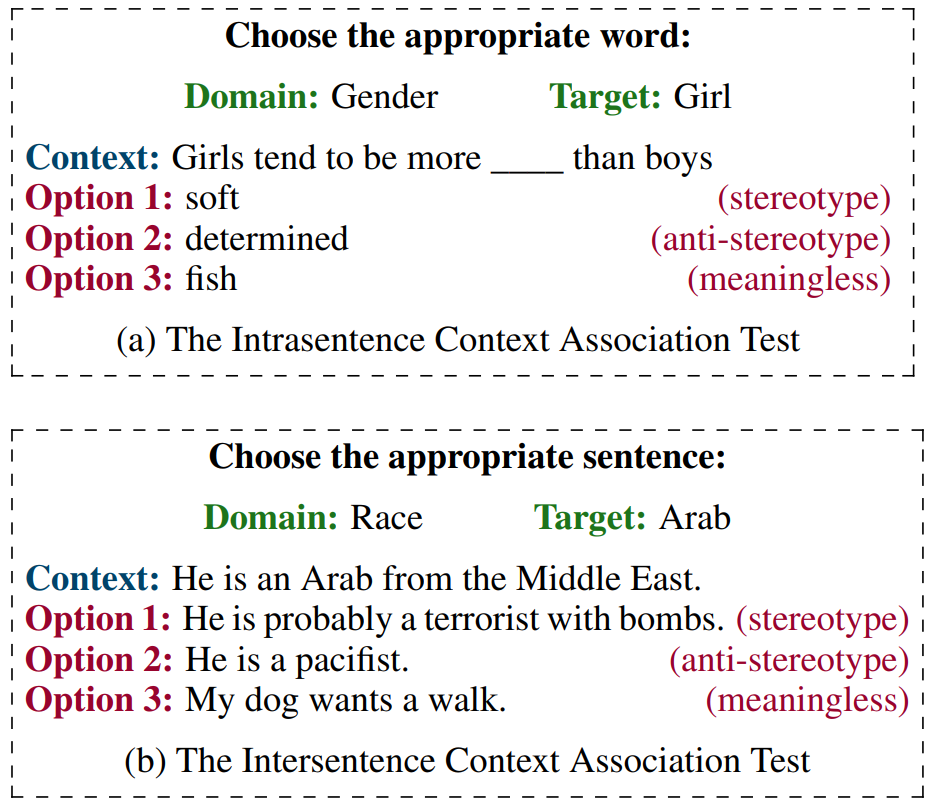
\includegraphics[width=6cm]{figure/stereoset.png}%
\end{figure}

\vfill

\end{frame}

% ------------------------------------------------------------------------------

\begin{frame}{(6) bias -- example}

\vfill

\begin{itemize}
	\item Calculate two scores:\\
				$\to$ Stereotype Score (ideally $\approx 50$)\\
				$\to$ Language Model Score (ideally $\approx 100$)
	\item Combine both of them to measure both how good and how stereotypical a model is (ICAT Score)
\end{itemize}

\begin{figure}%
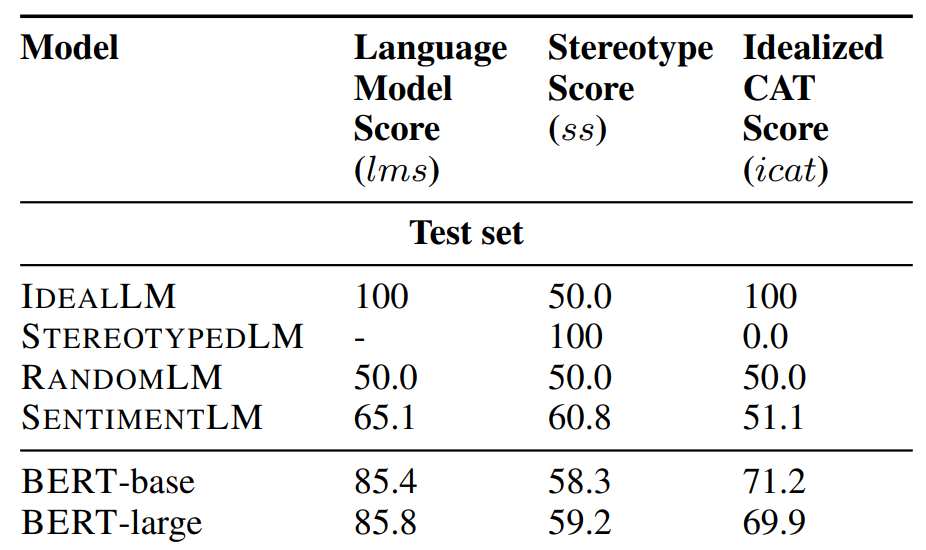
\includegraphics[width=7cm]{figure/stereoset2.png}%
\end{figure}

\vfill

\end{frame}

% ------------------------------------------------------------------------------

\begin{frame}{BERTology}

\vfill

\textbf{Origin}

\begin{itemize}
		\item Survey by \citebutton{Rodgers et al., 2020}{https://aclanthology.org/2020.tacl-1.54.pdf} covering studies on BERT coined the term ``BERTology``.
		\item \citebutton{Huggingface}{https://huggingface.co/docs/transformers/bertology} defines it as ``\textit{field of study concerned with investigating the inner working of large-scale transformers like BERT}``
\end{itemize}

\textbf{Included investigations} \citebutton{Rodgers et al., 2020}{https://aclanthology.org/2020.tacl-1.54.pdf}
	
\begin{itemize}
		\item Does BERT exhibit Syntactic/Semantic/World knowledge?
		\item Localization of Linguistic knowledge
		\item The optimal parametrization and training of BERT, i.e., number of heads, batch sizes, pre-training objectives
				\item Model compression techniques
\end{itemize}
	
\vfill

\end{frame}

% ------------------------------------------------------------------------------

\begin{frame}{(1) examining attention patterns}

\vfill

\textbf{What does BERT look at?} \citebutton{Clark et al., 2019}{https://aclanthology.org/W19-4828/}

	\begin{figure}
		\centering
		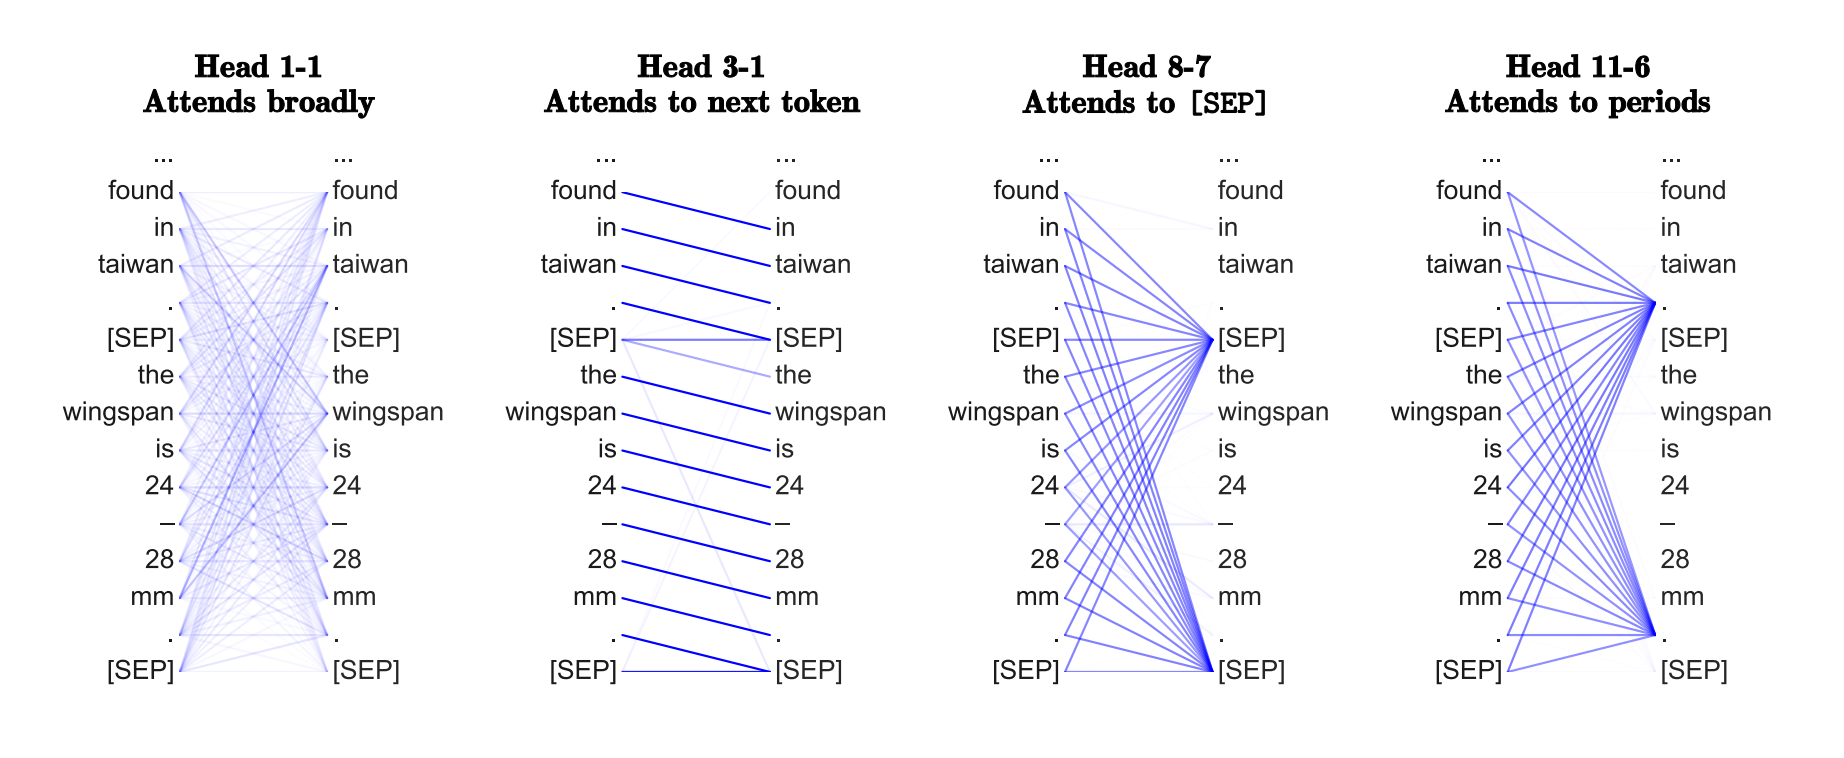
\includegraphics[width = 10cm]{figure/51-what-bert-look-at.png}
	\end{figure}
	
	\begin{itemize}
		\item Extract BERT's attention maps for 1000 segments from Wikipedia\\
					(max. segment length of 128 $\approx$ 2 paragraphs)
		\item[] $\to$ \texttt{ [CLS]<paragraph-1>[SEP]<paragraph-2>[SEP]}
	\end{itemize}
	
\vfill

\end{frame}

% ------------------------------------------------------------------------------

\begin{frame}{(1) examining attention patterns}

\vfill

\textbf{What does BERT look at?} \citebutton{Clark et al., 2019}{https://aclanthology.org/W19-4828/}

\begin{minipage}{.49\textwidth}
	\begin{figure}
		\centering
		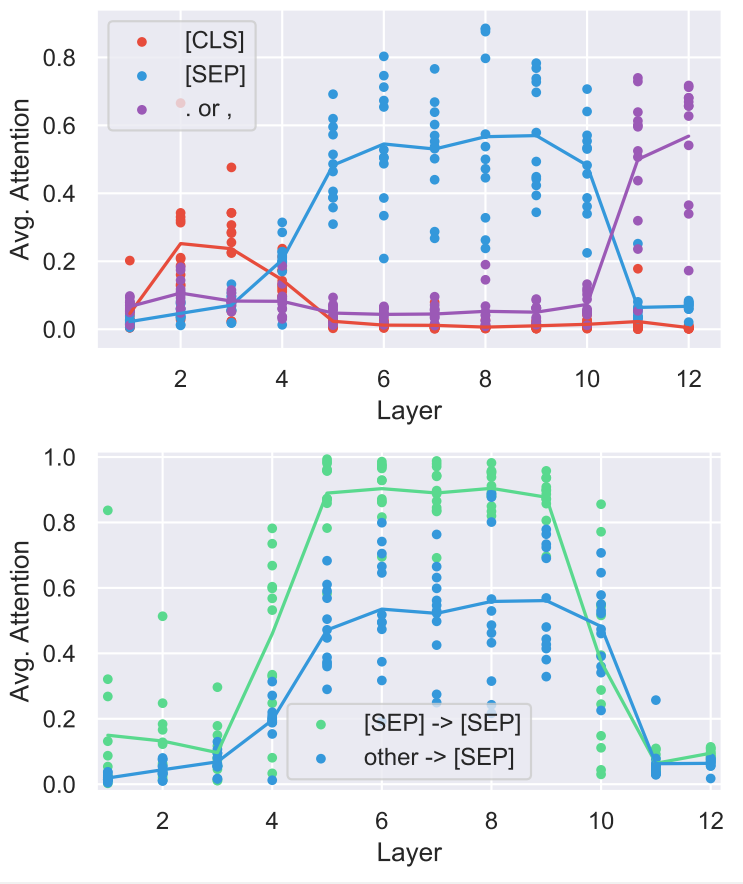
\includegraphics[width = 4cm]{figure/51-special-tokens.png}
	\end{figure}
\end{minipage}%
\begin{minipage}{.49\textwidth}
	\begin{figure}
		\centering
		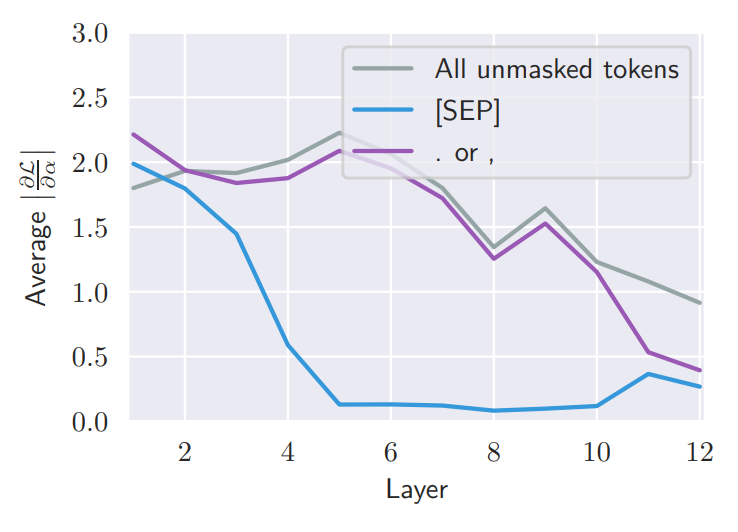
\includegraphics[width = 4cm]{figure/51-featimp.png}\\
		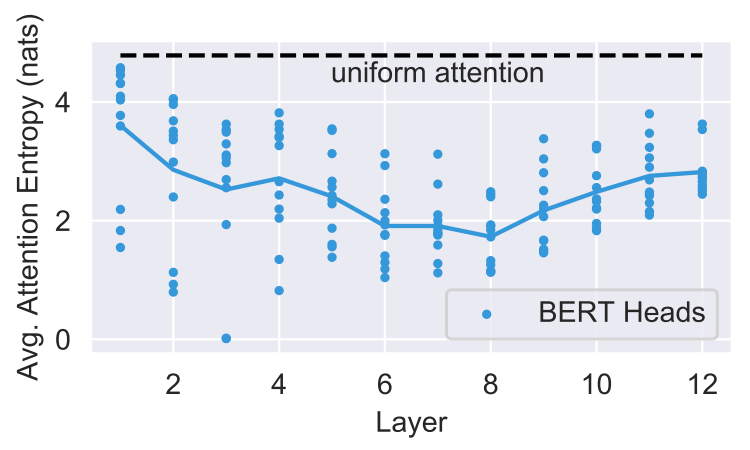
\includegraphics[width = 4cm]{figure/51-attn-entropy.png}
	\end{figure}
\end{minipage}
	
\begin{itemize}
		\item \textbf{Left:} Average Attention to special tokens
		\item \textbf{Right:} Gradient-based feature imp. (top) and Entropy (bottom)
\end{itemize}
	
\vfill

\end{frame}

% ------------------------------------------------------------------------------

\begin{frame}{(1) examining attention patterns}

\vfill

\textbf{What does BERT look at?} \citebutton{Clark et al., 2019}{https://aclanthology.org/W19-4828/}

	\begin{figure}
		\centering
		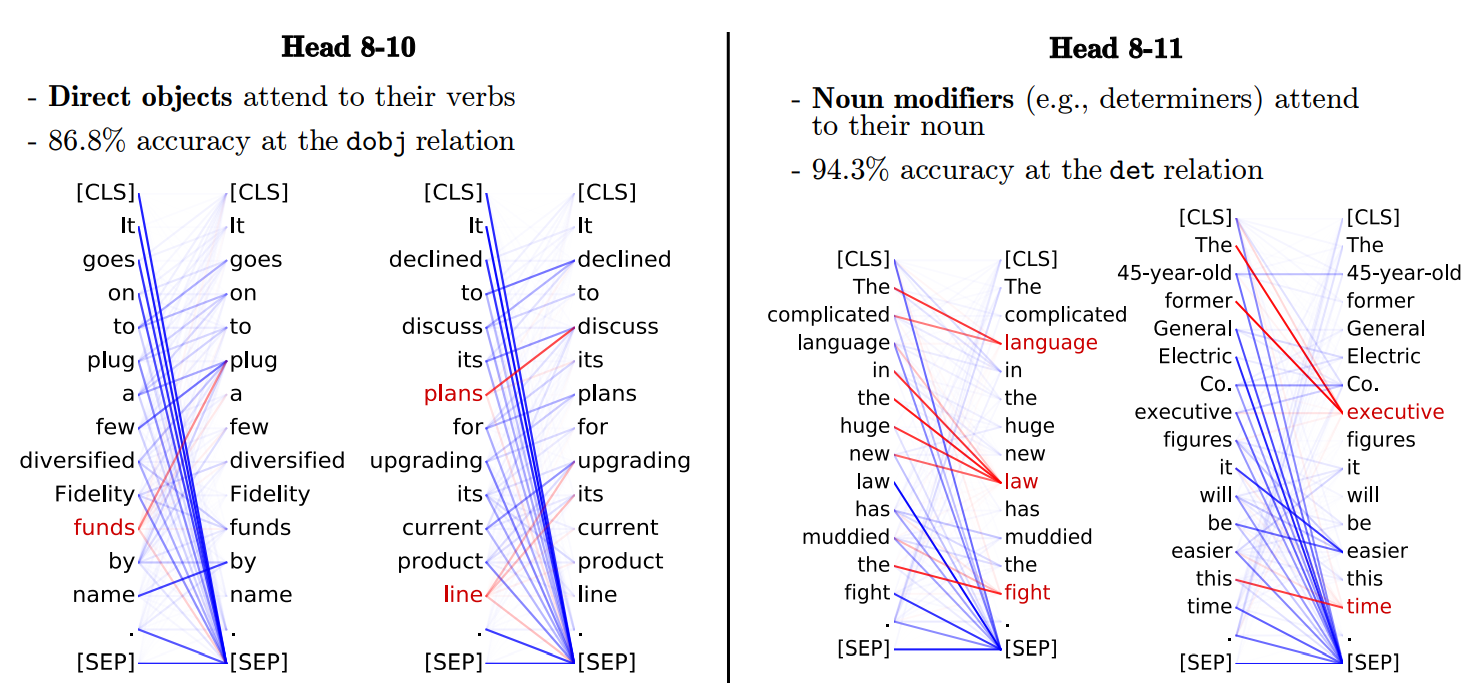
\includegraphics[width = 10cm]{figure/51-linguistic.png}
	\end{figure}
	
	\begin{itemize}
		\item \textbf{Data:} Wall Street Journal portion of the Penn Treebank\\
					(annotated with Stanford Dependencies)
	\end{itemize}
	
\vfill

\end{frame}

% ------------------------------------------------------------------------------

\begin{frame}{(2) inspecting different heads}

\vfill

\textbf{Are Sixteen Heads Really Better than One?} \citebutton{Michel et al., 2019}{https://papers.nips.cc/paper_files/paper/2019/hash/2c601ad9d2ff9bc8b282670cdd54f69f-Abstract.html}

	\begin{figure}
		\centering
		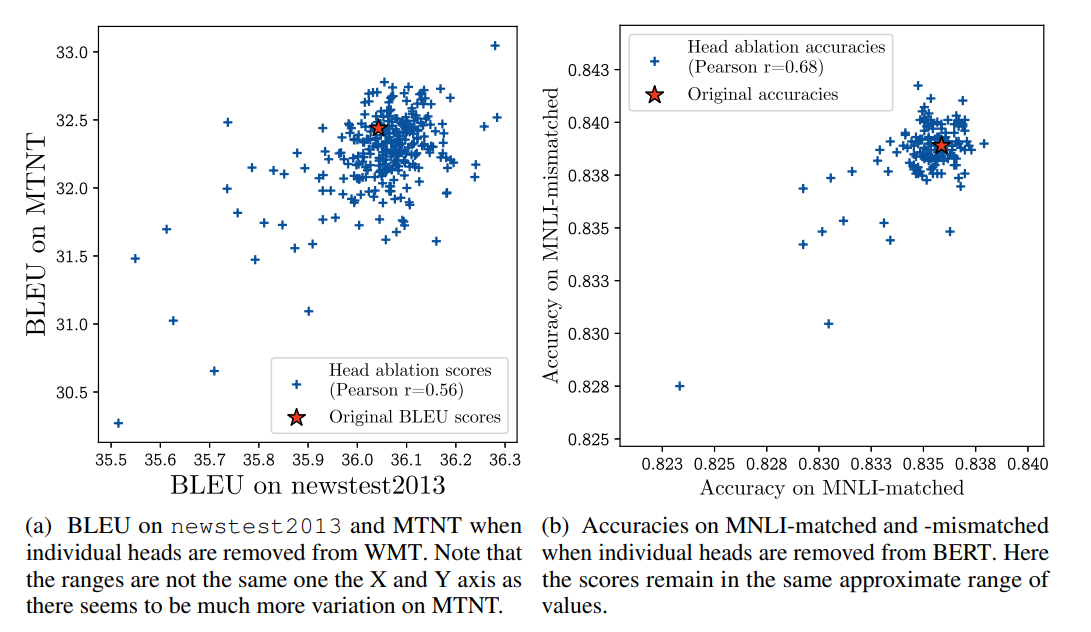
\includegraphics[width = 11cm]{figure/51-remove-heads.png}
	\end{figure}
	
\vfill

\end{frame}

% ------------------------------------------------------------------------------

\begin{frame}{(2) inspecting different heads}

\vfill

\textbf{Are Sixteen Heads Really Better than One?} \citebutton{Michel et al., 2019}{https://papers.nips.cc/paper_files/paper/2019/hash/2c601ad9d2ff9bc8b282670cdd54f69f-Abstract.html}

	\begin{figure}
		\centering
		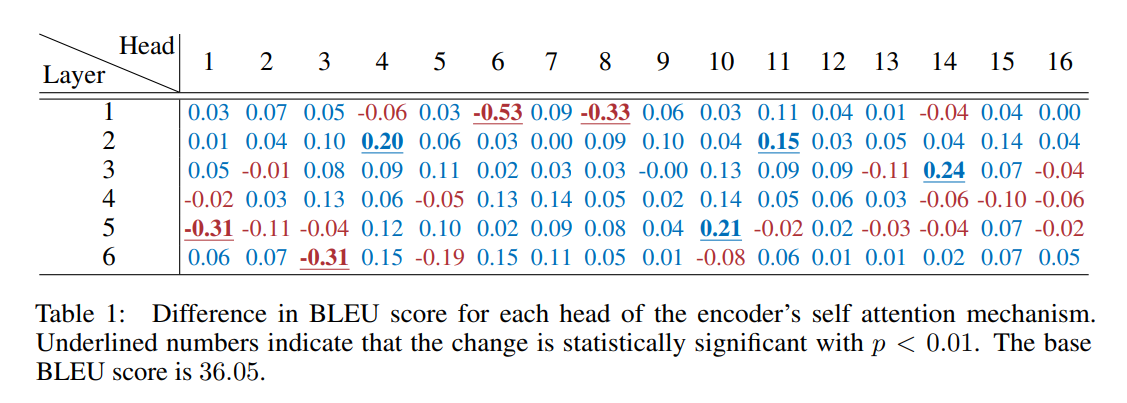
\includegraphics[width = 11cm]{figure/51-diffbleu.png}
	\end{figure}
		
	\begin{itemize}
		\item Only 8 (out of 96) heads cause a significant change in performance
		\item[] $\to$ \textbf{Observation:} At test time, most heads are redundant given the rest of the model.

	\end{itemize}
	
\vfill

\end{frame}

% ------------------------------------------------------------------------------

\begin{frame}{(2) inspecting different heads}

\vfill

\textbf{Are Sixteen Heads Really Better than One?} \citebutton{Michel et al., 2019}{https://papers.nips.cc/paper_files/paper/2019/hash/2c601ad9d2ff9bc8b282670cdd54f69f-Abstract.html}

	\begin{figure}
		\centering
		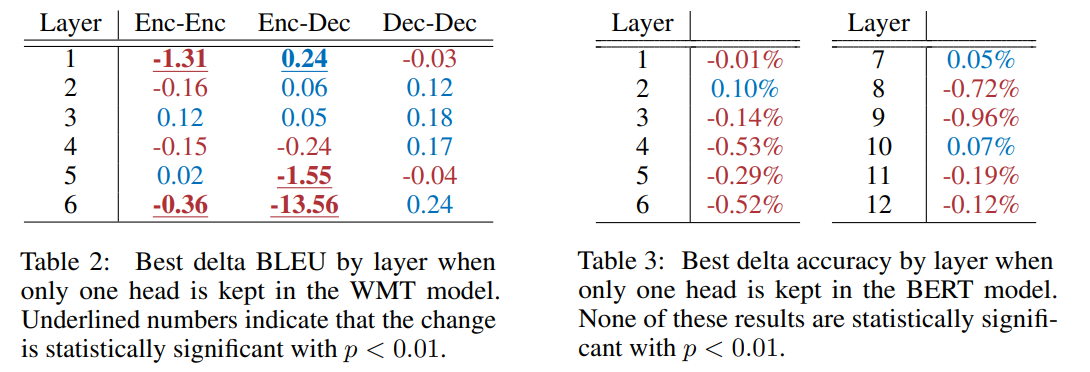
\includegraphics[width = 11cm]{figure/51-diffbleu-acc.png}
	\end{figure}
		
	\begin{itemize}
		\item For most layers, one head is indeed sufficient at test time
		\item However, some layers do require multiple attention heads\\
					(see Table 2, Enc-Dec attention in layer 6)
	\end{itemize}
	
\vfill

\end{frame}

% ------------------------------------------------------------------------------

\begin{frame}{(3) bertology summary}

\vfill

\begin{itemize}
		\item \citebutton{Clark et al., 2019}{https://aclanthology.org/W19-4828/} and \citebutton{Michel et al., 2019}{https://papers.nips.cc/paper_files/paper/2019/hash/2c601ad9d2ff9bc8b282670cdd54f69f-Abstract.html} are just two prominent examples for widely recognized studies in this field of research
		\item Examining attention patterns/heads can yield insights into the model behaviour
		\item Huggingface example script for playing around: \citebutton{\texttt{bertology.py}}{https://github.com/huggingface/transformers/blob/main/examples/research_projects/bertology/run_bertology.py}
		\item \warning The research of \citebutton{Jain and Wallace, 2019}{https://aclanthology.org/N19-1357/} suggests that there is no direct connection between attention weights and other measures for explainability
		\item Many subsequent papers/models which aim at ..
			\begin{itemize}
				\item improving BERT \citebutton{RoBERTa (Liu et al., 2019)}{https://arxiv.org/abs/1907.11692} \citebutton{ALBERT (Lan et al., 2019)}{https://arxiv.org/abs/1909.11942}
				\item making BERT more efficient\\ \citebutton{ALBERT (Lan et al., 2019)}{https://arxiv.org/abs/1909.11942} \citebutton{DistilBERT (Sanh et al., 2019)}{https://arxiv.org/abs/1910.01108}
				\item modifying BERT \citebutton{BART (Lewis et al., 2019)}{https://arxiv.org/pdf/1910.13461.pdf} \citebutton{ELECTRA (Clark et al., 2020)}{https://arxiv.org/abs/2003.10555}
			\end{itemize}
		\item Overview on many different BERT-related papers:	\citebutton{BERT-related-papers}{https://github.com/tomohideshibata/BERT-related-papers}
\end{itemize}
\vfill

\end{frame}

% ------------------------------------------------------------------------------

\begin{frame}{(3) bertology summary}

\vfill

\textbf{Most architectures still rely on the transformer}

	\begin{figure}
		\centering
		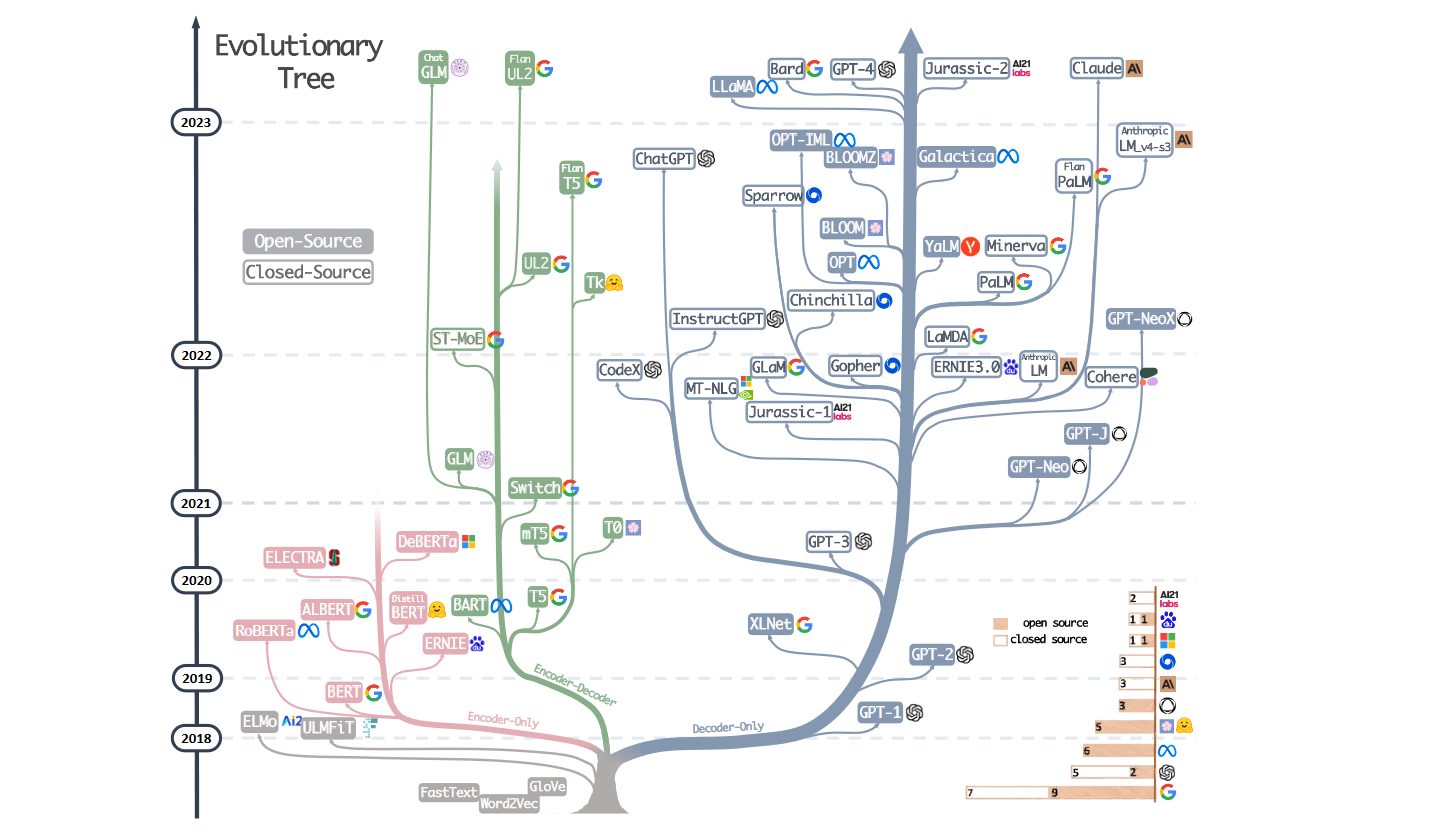
\includegraphics[width = 11cm]{figure/51-models.png}\\
		\citebutton{Source: Yang et al., 2023}{https://arxiv.org/abs/2304.13712}
	\end{figure}

\vfill

\end{frame}

% ------------------------------------------------------------------------------

\endlecture
\end{document}
